\subsection{Introducción}
Las técnicas de \textit{Spreading Activation}, en adelante \textit{SA}, nacieron en el campo
de la Psicología~\cite{AndersonTheory,Collins_Loftus_1975}, como resultado de la investigación de la
memoria humana y, más especialmente, en la búsqueda de
procedimientos para explotar las formas de representación del
conocimiento humano.


Estas técnicas intentan ``simular'' el comportamiento de la memoria humana y
generar una navegación conceptual con significado de la misma manera que lo
haría nuestra propia memoria. Para ello hay que comprender cuales son las maneras de
asociar el
``significado'' (memoria semántica), la diferencia entre ellas reside con tipo
de organización (relación entre los elementos semánticos) y con el grado de
conexión que se establecen entre las palabras y la realidad externa, es decir,
entre el nivel conceptual perceptivo a través del cual percibimos el mundo sobre
el que hablamos y que somos capaces de procesar.
\begin{description}

 \item[Semántica procedimental:] esta teoría especifica el significado de las
 palabras teniendo en cuenta su relación con el mundo (las dos siguientes teorías
 prescinden del mundo para obtener el significado de las palabras). Tiene en cuenta tanto
 el conocimiento intensional como el extensional.

\item[Rasgos semánticos:] las teorías de este grupo asocian al significado de
las palabras una definición. En cada definición, encontramos otras palabras que
pueden considerarse como elementos constitutivos del significado de la palabra
definida, constituyendo los elementos básicos de significado o ``marcadores semánticos''.

 Comprender una palabra conllevaría acceder a la lista de  ``marcadores
 semánticos''. En este grupo se encontraría la teoría de marcadores semánticos de
 \textit{Chomsky}.
 
 
 \item[Redes semánticas\footnote{Punto de vista de la Psicología}:] el interés primordial
 no es conocer cuáles son las
 notas distintivas de un determinado concepto sino saber el tipo de organización
 de las representaciones semánticas. El significado de las palabras (conceptos)
 está representado por las relaciones de pertenencia o inclusión y las de
 posesión con los demás conceptos. Aparte de las relaciones entre categorías o
 clases existen las de ``posesión'' que expresan las propiedades de cada uno de
 los conceptos.
 
 Es preciso tener en cuenta que la información no es nunca ``redundante''
 (``economía cognitiva''),
 las propiedades de un nodo o concepto de nivel superior no se repiten en los
 inferiores ya que se heredan.
\end{description}


Dentro de la Web Semántica y teniendo en cuenta el uso de las ontologías
como base de conocimiento, se pueden ver como un tipo especial de red semántica
 que formaliza las relaciones entre los conceptos utilizando una lógica
 determinada y que, por lo tanto, simula el comportamiento de la memoria o del
 conocimiento humano, ya que plasma el conocimiento de un dominio (de un
 humano) sobre una estructura lógica.
 
\subsubsection{Necesidad computacional}

La representación del conocimiento utilizando un conjunto de conceptos relacionados entre sí se 
adapta perfectamente al mundo real. En el conjunto de estos conceptos, encontramos tanto datos 
y relaciones de carácter general, como conocimiento específico dentro de un dominio concreto. 
Por ello, se hace especialmente interesante proveer a las aplicaciones de un método para 
obtener un conjunto de conceptos relacionados entre sí de forma automática.

Los algoritmos normalmente utilizados para realizar estas exploraciones se basan en 
métodos de búsqueda sobre redes semánticas, o basados en 
redes neuronales\cite{Chen95}. La principal diferencia es la forma en la cual 
representan el conocimiento y la capacidad de expresividad semántica:


\begin{description}
\item [Redes semánticas\footnote{Punto de vista computacional}:]  utiliza nodos para
representar conceptos, entidades o
 clases y mediante flechas indicamos las relaciones existentes entre ellos, 
pudiendo marcar estos enlaces con distinta información como pesos o etiquetas. 
Alta expresividad semántica a través de las relaciones.

\item [Redes neuronales:] los nodos o neuronas y sus conexiones intentan asemejar el 
conocimiento a la representación cerebral, se utilizan patrones de activación 
para indicar el estado de las neuronas y conexiones de la red. 
Escasa expresividad, métodos numéricos.
\end{description}


Una vez que se elige una forma de representación, debemos disponer de un método 
sistemático y eficaz para la exploración. En redes semánticas lo habitual suele ser 
utilizar algoritmos basados en \textit{Brand and Bounch} para el tratamiento de grafos
que se caracterizan por su eficiencia, para redes neuronales consistirá 
en distinguir con que grado son activados los conceptos y actuar en
consecuencia.
 
 
\subsubsection{\textit{Spreading Activation}}

El modelo básico de \textit{SA} consiste en una
una red de nodos interconectados, un grafo. Si los nodos representan
objetos o clases del dominio y los arcos, relaciones que se
establecen entre ellos, podemos hablar entonces de una red
semántica. El procesamiento realizado por el algoritmo se basa en un
método de exploración de grafos utilizando un modelo iterativo. Cada
una de las iteraciones se compone de una serie de pulsos y condición
de parada, en los que cada pulso está formado, a su vez, por
distintos pasos de ejecución.
\medskip

La utilización de \textit{SA} como algoritmo de
exploración de grafos no es nueva y ya a principios de los años
80\cite{Scott1981} aparecían los primeros trabajos de investigación
nombrando a este algoritmo. Como antecedentes podríamos nombrar
trabajos en torno a redes neuronales, redes semánticas y a los
algoritmos clásicos de búsqueda en grafos. Su uso se centra
principalmente en el campo de ``Information Retrieval''\cite{SpreadingActivationIR,Helmut2004} y ``Document
Retrieval''\cite{turtle91inference}. Aunque con el apabullante éxito
de Internet en los últimos años, el uso de este algoritmo ha
derivado en obtener documentos de hipertexto\cite{Agosti1993} o
multimedia de la red. Por otra parte, y más parecido al enfoque que
pretendemos dar, encontramos trabajos relacionados con un procesos
de búsqueda híbridos\cite{RochaSA04,Qiu93,conf-sofsem-Suchal08,Schumacher+2008search} en los que se intenta generar
una consulta sintáctica basada en la exploración previa de una base
de conocimiento~\cite{XueHYZCM04}. Hoy en día y debido al gran 
éxito de las redes sociales y la necesidad de explotar
la información que los usuarios van creando continuamente se ha
utilizado está técnica para realizar anotaciones semi-automáticas~\cite{Chen:2007:PSA:1780653.1780702,GelgiVD05}, 
análisis de opiniones~\cite{paper:troussov:2008} o 
recomendaciones a los usuarios~\cite{citeulike:3779904,gouws-vanrooyen-engelbrecht:2010:CCSR}.

En el campo de Linked Data también está teniendo cabida como consecuencia
del ``grafo'' subyacente a esta iniciativa y cuya explotación de forma eficiente~\cite{Grinberg:2011:ASA:1940632.1940674}
resulta de gran interés para las aplicaciones. 


\medskip



\subsubsection{Ontologías y \textit{Spreading Activation}}

 Aunque, como hemos comentado,  una representación basada en ontologías
 formalmente no constituye una red semántica propiamente dicha, si se puede ver
 como tal la estructura de clases y relaciones definidas. 
La analogía subyacente reside entre las clases (también válido para instancias) 
con nodos, y relaciones con arcos. De esta manera la activación de conceptos o clases y 
sus relaciones dentro de una ontología se puede asimilar al modelo que 
utilizaríamos en el caso de una red semántica. Las técnicas basadas en 
\textit{Spreading  Activation} se han establecido como las más adecuadas para la exploración 
de esquemas conceptuales~\cite{DBLP:journals/cogsr/KatiforiVD10,DBLP:journals/ijsc/DixKLVS10,liu_et_al_2005}, en contraposición a las basadas en teorías clásicas de grafos y algoritmia. 

Este conjunto de técnicas, por lo tanto,  resultan atractivas para ser aplicadas
sobre las ontologías de dominio, a los conceptos que constituyen un
ámbito particular de conocimiento con el objetivo de obtener un conjunto ponderado de
conceptos relevantes según un determinado conjunto de entrada.


\subsubsection{Definición del algoritmo}

Las técnicas de \textit{SA} son un método para
explorar redes semánticas a partir de un conjunto incial de
conceptos con determinada puntuación asociada A partir de este
conjunto, la ``activación'' se propaga iterativamente a los demás
conceptos relacionados con ese conjunto inicial. Los ``pesos'' de
los conceptos suelen ser valores reales que decrecen según la
activación se propaga por el grafo. Los valores asociados a la
entrada de los nodos y los pesos de las relaciones entre los
conceptos son configurables dependiendo de la aplicación. A los
efectos de que se formen núcleos de activación, los pesos de ls
relaciones deben ser menores que 1. Evidentemente, esto modificará
también su interpretación. La implementación del algoritmo se divide
en las siguientes fases,


\begin{figure}[h]
 \centering
 %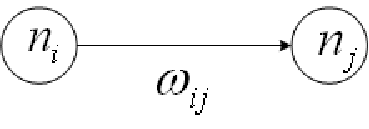
\includegraphics[width=4.8cm]{images/spreading}
    \caption{Modelo gráfico del \textit{Spreading Activation}}
 \label{fig:spreading}
\end{figure}





\begin{description}
\item [Ajuste previo (\textit{preadjustement}):] esta fase inicial, de carácter opcional, se
 suele utilizar para realizar alguna estrategia de control sobre el
 grafo que se va a explorar.
\medskip

\item [Propagación (\textit{spreading}):] fase de expansión del
algoritmo. Los conceptos se van activando por oleadas, en las que el
nodo tratado activa a sus nodos vecinos.
\medskip


El cálculo del grado de activación $I_i$ de un nodo $n_i$ se realiza
mediante la fórmula:

\begin{equation}
I_i  = \sum_j{O_j \omega_{ji}}
\end{equation}
\medskip




Donde $I_i$ es el total de entradas del nodo $n_i$, $O_j$
es la salida del nodo $n_j$ conectado al nodo $n_i$ y $\omega_{ji}$
es el peso de la asociación del nodo $n_j$ con el nodo $n_i$. Si no
existe relación entre el nodo $n_j$ y el nodo $n_i$ se asume que
$\omega_{ji} = 0$.  Más adelante se discute cómo se calcula el valor
de salida $O_j$ de un nodo $n_j$ a partir de su valor de entrada $I_j$.
\medskip


Para evaluar el ``peso'' de un nodo y decidir si un concepto está
activo o no, se utiliza una función $f$ de evaluación de activación
definida como:

\begin{equation}
\label{equ:activation} N_i = f(I_i)
\end{equation}
\medskip


La función de activación $f$ puede devolver diferentes valores
dependiendo nuevamente del ámbito de la aplicación y de la
interpretación que queramos asignar a este valor. No obstante, el
caso más habitual es considerar como posibles valores $N_i$, $1$ y
$0$, que indican si el nodo ha sido activado o no respectivamente:


\begin{equation}
N_i=f(I_i)=\begin{cases} 0 & \text{si $I_i < \jmath_i$} \\ 1 &
\text{si $I_i
> \jmath_i$}
\\ \end{cases}
\end{equation}
\medskip


Denotamos por $\jmath_i$ el valor de activación umbral para $i$.
Este valor $\jmath_i$ es dependiente de la aplicación y es habitual
que varíe de un nodo a otro, aunque también puede ser constante. Hay
que tener en cuenta que el grado de activación $I_i$ de un nodo
$n_i$, a medida que se vaya iterando el algoritmo, puede ir
cambiando.


\begin{figure}[h]
 \centering
 %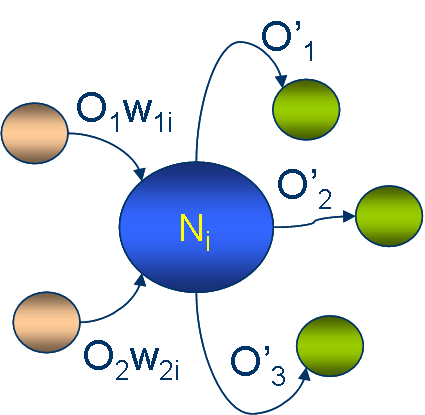
\includegraphics[width=6cm]{images/modelo-sa}
    \caption{Activación de conceptos en \textit{Spreading Activation}}
 \label{fig:modelo-sa}
\end{figure}




\medskip
Una vez que se satisfaga la regla de terminación, bien por número de
iteraciones $k$ o por otras restricciones establecidas como un valor
mínimo de activación, el algoritmo finalizará devolviendo un
conjunto de nodos $\mathcal{G}^k$ y para cada nodo $n_i$ un peso o
grado de activación $I_i$, es decir, un conjunto constituido por
pares ordenados de la forma $(n_i, I_i)$.
\medskip


\item [Ajuste posterior (\textit{postadjustment}):] es la fase final. Está destinada al control de los conceptos activados y es opcional.

\end{description}


%
 \subsection{Parametrización del \textit{Spreading Activation}}\label{restricciones}
%
El algoritmo de propagación se carateriza por su flexibilidad desde
el punto de vista de la configuración. Por eso, se han establecido
una serie de restricciones\cite{Cohen1987} como mejoras del
algoritmo para ajustar los resultados de la activación de conceptos
a cada caso de aplicación, y que no se produzcan valores erróneos.
\medskip
\begin{description}

 \item [Distancia:]

Los nodos que se encuentren alejados de un nodo activado deberían
ser penalizados ya que es necesario realizar muchos saltos para
poder llegar a activarlos.

\begin{definition}
 La distancia del nodo $n_j$ al nodo $n_i$, $d_{ji}$, en una red conceptual es
  el número mínimo de vértices que deben recorrerse para llegar del nodo $n_j$ al $n_i$.
\end{definition}


\medskip

\item[Camino:]
El camino seguido por la activación desde un nodo puede ser guiado
atendiendo a los pesos y a las etiquetas de las relaciones.
Nuevamente, esta característica se configura dependiendo de la
aplicación con el objetivo de afinar los resultados de la
propagación obtenidos.


\item[Múltiples salidas (Fan-Out):]

Los Nodos ``altamente conectados'', con muchas relaciones de salida
con otros nodos,
pueden desvirtuar el objetivo de la propagación
activando nodos que probablemente no se encuentran en el conjunto de
activación deseado. Se configura entonces un umbral para determinar
el nivel de conectividad máximo permitido para la activación del
nodo y su propagación.
\begin{note}
Un nodo $n_i$ será activado con el peso correspondient $I_i$ si su
grado de salida, $g_i$, el número de arcos que salen de $n_i$, es
inferior una a constante umbral $\ell$.
 \end{note}


\item[Umbral de activación:] Como comentamos en la fase de
\textit{Spreading} de definición del algoritmo, se puede
parametrizar la activación de un nodo a partir de un valor umbral
mínimo establecido y una función $f$ de evaluación de la activación.
Si el valor de activación de un nodo está por debajo del valor
umbral mínimo establecido este nodo no debería ser propagado.

\begin{note}
Un nodo $n_i$ será propagado sii su valor de activación, $I_i$, es
mayor que una constante umbral de activación $\jmath$.
 \end{note}


\end{description}



La aplicación de estas restricciones simplifica y restringe el
algoritmo de \textit{SA}, permitiendo la
adaptación a problemas concretos y afinando los valores de
activación de los conceptos.



\subsection{Implementación de \textit{Spreading Activation}}


El uso de las técnicas de \textit{SA} se aplica para, a partir
de los conceptos de la consulta inicial del usuario ($Q_{sem}$), extraer un
nuevo conjunto de conceptos relevantes ($Q'_{sem}$) que permitan
construir una ``\textit{query} enriquecida'' con terminología de
dominio ($Q'_{sin}$). Los conceptos están organizados en un sistema
de ontologías, donde cada ontología $O_i$ formaliza y modela un
dominio determinado $\mathbb{D}_i$.

\medskip

Las ontologías son sistemas de representación de conocimiento que,
estructuralmente, podemos contemplar como una {\bf red semántica},
por tanto, como un grafo donde cada nodo $n_i$ representa un
concepto $c_i$ de la ontología de dominio y el arco $\omega_{ji}$ la
relación semántica entre los conceptos $c_j$ y $c_i$. La terminación
del algoritmo ofrece como resultado el conjunto de pares ordenados
$(n_i, I_i)$ que forman $Q'_{sem}$, donde $n_i\approx c_i$ y
$I_i\approx w_i$, la relevancia del concepto.

\medskip
Una arquitectura basada en ontologías propone un modelo en el cual los
conceptos pueden pertencer a varios dominios, en la que el valor
semántico de un concepto (las propiedades que lo definen) puede
variar de un dominio a otro. Por ello, la consulta de un usuario es
válida si todos los conceptos pertenecen al mismo dominio
$\mathbb{D}_{com}$. Así el lanzamiento del algoritmo de activación
de conceptos sólo se realiza en el dominio $\mathbb{D}_{com}$
seleccionado a partir de la consulta del usuario. El objetivo de
esta restricción será obtener conceptos
   relevantes en el ámbito que estamos buscando, de esta forma el conjunto
    de conceptos de salida es siempre semánticamente correcto. Nos encontramos
     ante una condición necesaria de activación y propagación.

\begin{definition}
Sea $\mathbb{D}_{com}$ el dominio activo para una búsqueda, si un
concepto $c_i$ es activado y propagado, entonces $c_{i} \in
\mathbb{D}_{com}$.
\end{definition}

\medskip

Por ejemplo, el objetivo de utilizar estas técnicas de activación es seleccionar
un conjunto adecuado de conceptos para la localización de documentos
cercanos a los intereses de los ciudadanos que consultan el BOPA. La
exploración de la ontología como una red semántica nos permite
extraer a partir de la consulta del usuario (que refleja en algún
sentido sus objetivos de búsqueda) conceptos cercanos que, gracias a
la semántica estructural del dominio, serán relevantes para
enriquecer la consulta original con conocimiento experto y generar
un conjunto de términos completamente adaptados al vocabulario
normativo de los documentos oficiales.

\medskip
La implementación del \textit{SA} consiste en
construir dos conjuntos de conceptos que guardan información sobre
el estado del algoritmo. Para su definición, tenemos que
$\mathbb{D}_{com}$ es el conjunto de conceptos de la red semántica,
$\Phi$\footnote{$\Phi$ y $Q_{sem}$ son el mismo conjunto.} es el
conjunto de conceptos inicialmente activados, $c_j^k$ es un concepto
propagado en la iteración $k$-ésima (a partir de él se activan otros
conceptos) y, por último, $\omega_{ji}^k$ es la relación por la que
se propaga el algoritmo desde $c_j^k$ hasta $c_i$ en la iteración
$k$-ésima:

\begin{description}



\item [Conjunto $\mathcal{A}$:] cola de conceptos {\bf activados} candidatos a ser propagados. Formalmente
podemos describirlos de la siguiente manera:


\begin{align}
 \mathcal{A}^0 &=\Phi \\
 \mathcal{A}^k &=(\mathcal{A}^{k-1} \cup \{c_i: {\forall c_i /  \omega_{ji}^k >0}\})-{ \{\mathcal{G}^k}\}
\end{align}



\item [Conjunto $\mathcal{G}$:] conjunto de conceptos propagados:

\begin{align}
 \mathcal{G}^0 &=\emptyset \\
 \mathcal{G}^k &= \mathcal{G}^{k-1} \cup \{c_j^k\}
\end{align}

donde el \textit{output} del algoritmo es  el conjunto de conceptos
ponderados que representa la nueva consulta enriquecida:
$\mathcal{G}^k = Q'_{sem}$.


\end{description}

\medskip

Por último, podemos definir el cálculo de la activación de un
concepto $c_i$ en la iteración $k$, denotado por $I^k_i$. En la
iteración $0$ podemos calcular el valor de activación de $c_i$ como:
\begin{equation}
I^0_i=\begin{cases}%
  1 & \text{si $c_i \in \Phi$} \\%
  0 & \text{si $c_i \notin \Phi$} \\%
 \end{cases}
\end{equation}

en la iteración $k$, calculamos el valor de activación $c_i$ a
partir del elemento $c_j^{k}$ desde el que se activa.


\begin{equation}
I^k_i=\begin{cases}%
  I^{k-1}_i & \text{si } \omega_{ji}^k = 0 \\%
  I^{k-1}_i + \omega_{ji}^k I^{k-1}_j  & \text{si }  \omega_{ji}^k > 0  \\%
 \end{cases}
\end{equation}


\subsubsection{Validación de \textit{Spreading Activation}}

La definición de este algoritmo le exime de ser aplicable como
técnica para la búsqueda en espacios de estados, como $A^*$, ya que aunque cuenta
con un estado inicial (conjunto de conceptos de entrada) conocido, el estado
final (conjunto de conceptos ponderados) no se formula como un objetivo del algoritmo,
simplemente se consigue por ejecución del mismo y como finalización a un proceso limitado por una serie de
restricciones. Ahora bien, es necesario asegurar la computabilidad en tiempo
finito, por razones obvias, del algoritmo. Al igual que en los algoritmos
clásicos de búsqueda sobre grafos se realiza una descripción de sus
caracterísicas computables vamos a realizar una descripción análoga para
\textit{SA}.

\begin{definition}
Un algoritmo de búsqueda es completo si termina con una solución siempre que
ésta exista.
\end{definition}

Aplicando esta definición a \textit{SA}, el algoritmo es
\textit{completo} ya que siempre existe un estado final (conjunto de conceptos
ponderados) desde un estado inicial. Independientemente de las iteraciones
ejecutadas por el algoritmo siempre se obtendrá una salida.

Además, podemos asegurar que siempre va a terminar por dos razones:
\begin{itemize}
  \item las restricciones básicas, figura \ref{restricciones}, que dispongamos como  
  condición de parada en algún momento se cumplirán, terminando la ejecución.
   \item en algún momento determinado en la ejecución no existirán conceptos
   para propagar $\mathcal{A} = \emptyset$, con lo cual el algoritmo finalizará.
\end{itemize}  

\begin{note}
Si en la inclusión de nuevas restricciones de parada no podemos asegurar la
finalización algoritmo, deberemos adaptarlas para su ejecución con las
restricciones básicas que siempre nos aseguran la ejecución en tiempo finito del
algoritmo.
\end{note}


\begin{definition}
Un algoritmo es admisible si devuelve una solución óptima (con camino desde el
estado inicial con coste mínimo) cuando exista solución.
\end{definition}

En este caso, no podemos asegurar que el algoritmo sea ``admisible'' ya que los
resultados dependerán del conjunto de entrada, de los pesos de las relaciones,
de la función de degradación, de la definición de las restricciones, de la base
de conocimiento, etc.
Es decir, encontrar la combinación óptima de todos estos parámetros (que siempre
genere una salida óptima) para generar un
estado final óptimo, es en la práctica imposible. 
Hay que tener en cuenta que no se dispone de una función que nos indique la
``bondad'' de un nodo y como tampoco se dispone de un estado final prefijado (no
es un algoritmo de búsqueda) no podemos decidir si es o no ``admisible''. 


Debe apuntarse que tanto la validación y ajuste de los parámetros del algoritmo
debería realizarse por expertos del dominio sobre los que se ejecuta la técnica
de activación/propagación. La genericidad y flexibilidad del algoritmo generan
soluciones ``aceptables'' o suficientemente buenas (según configuración) para casi cualquier
dominio o problemas que no requieran optimización de la solución. 


\subsection{Versión de \textit{Spreading Activation}}\label{sect:version-sa}
%

Aunque aún resta trabajo en el control de la activación de los conceptos, se
estima que las características que pueden tener mayor implicación en la mejora
del algoritmo son las siguientes:


\begin{itemize}
\item Esquema conceptual sobre el que se trabaja.
\item Diseño de las relaciones entre conceptos: ponderación y etiquetado.
\item Tamaño de la propagación.
\item Granularidad de los resultados de búsqueda.
\item Dificultad de implementación.
\item Evaluación de mejora conseguida como aplicación de las nuevas características.
\end{itemize}

Los esfuerzos se concentran actualmente en los
siguientes puntos:

\begin{description}

\item[Contexto de activación:] de cara a aplicaciones reales de uso del
algoritmo puede resultar interesante establecer un determinado contexto de
activación para los conceptos de una determinada ontología. En el diseño y
construcción de ontologías se hace uso habitualmente del reaprovechamiento de
conocimiento ya definido, es decir, utilizar conceptos ya definidos para generar
nuevas bases de conocimiento agregado. En estos casos, puede ser que los
conceptos reutilizados no sean de interés para un dominio concreto y en esta
situación los únicos conceptos que deberían activarse y propagarse deberían ser
los pertenencientes a un determinado contexto $C$, descartando los demás por su
escasa transcendencia. Estos nodos o conceptos descartados simplemente se deben
usar como puente para la propagación de conceptos pertenencientes a $C$. En
cuanto a su implementación y atendiendo al concepto de URI y espacio de nombres
en la Web Semántica, definiremos el contexto de activación $C$ como un espacio
de nombres $C_{ns}$ de determinada URI $C_{uri}$ y de acuerdo a esto sólo se propagarán
los conceptos que pertenezcan ese $C_{ns}$.


No obstante, para completar la definición de esta restricción hay que realizar
una apreciación para mantener la computabilidad finita de todas las restricciones y
por tanto del algoritmo. Imaginemos una configuración del algoritmo que sólo
tenga en cuenta esta restricción, el algoritmo acogería un carácter infinito:
buscando nodos que pertenezcan $C_{ns}$, el algoritmo podría ``saltar''
entre ontologías en búsqueda de nodos aptos para propagar sin éxito y podría
darse el caso de que nunca acabara. 
Para evitar estas situaciones se ha establecido una  cota máxima de rechazos
$C_{retries}$ al contexto $C$, de esta forma si se  formulan más peticiones
fallidas de propagación que las determinadas en el contexto el  algoritmo
mantiene su propiedad de convergencia. 
 
 Un valor inicial para esta  cota puede ser el número de conceptos del espacio
 de nombres, quedando a  elección del conocimiento este valor y teniendo en
 cuenta que el algoritmo  podría adquirir un carácter infinito activando y
 propagando nodos que pertenezcan al $C_{ns}$ establecido, quedando patente  que
 esta situación compromete el tiempo de ejecución del algoritmo, aparte de la
distorsión de los resultados.

  

\item[Control de tiempo $t$ de activación:] este tipo de restricción se define como
el tiempo $t$ mientras el cual se activan conceptos. La inclusión de esta
restricción se debe principalmente a razones de ejecución automática del
algoritmo para la obtención de resultados de evaluación. La idea es imponer un
tiempo de activación global y cada vez que un concepto se propague activando
nuevos conceptos ir acumulando este tiempo de activación para poder establecer
rangos de tiempo en los cuales el algoritmo se pueda ejecutar independientemente
de otras restricciones. Desde un punto de vista semántico, esta restricción no
tiene ningún valor, pero en cambio funcionalmente representa metainformación
sobre la ejecución del algoritmo que nos puede facilitar la bondad de una
ejecución $k$ del algoritmo. Por ejemplo, podemos establecer que un determinado
porcentaje de los casos las ejecuciones por debajo de cierto tiempo $t_k$ han
presentado resultados aceptables en términos de activación de conceptos y tamaño
del conjunto de salida. 

\item[Degradación de la salida $O_j$:] trabajando en una versión del
modelo genérico del \textit{SA}, para aplicar
algunas restricciones que mejoren su comportamiento y, por tanto,
los resultados obtenidos. Actualmente, es necesario seguir investigando en una
redefinición del cálculo del valor de activación a partir de una
función $h$ que degrada el valor de salida $O_j$ de un concepto
$c_j$:



\begin{itemize}

\item Parametrización genérica: Esta función $h$ de degradación permite
obtener la salida de un concepto $c_j$ a partir de su grado de
activación:

\begin{equation}
O_j = h(I_j)
\end{equation}



\item Caso básico: Cuando la función $h_0$ es igual que la función identidad, $h_0 = id$, la salida
$O_j$ toma como valor el nivel de activación del concepto
$c_j$:

\begin{equation}
O_j = h_0(I_j) = I_j
\end{equation}



\item Parametrización usando {\bf distancia}: Como el nivel de activación de un
concepto $n_j$ que ha sido activado desde un concepto inicial $n_l$
(perteneciente a $\Phi$) depende de la distancia del concepto $n_l$
al concepto $n_j$, cuanto más nos alejemos de $\Phi$, la puntuación
debe ir decayendo, de forma que para el camino que recorre el
algoritmo desde $n_l$ hasta $n_j$: $I_l > I_j$.

\medskip
La función $h_1$ degrada la salida de los conceptos de forma que
disminuye la puntuación de aquellos conceptos que se alejan del
``núcleo de activación'' y premia cuán cerca esté un concepto de los
nodos originales. Así que dada la distancia $d_j$, donde $d_j = min
\{d_{lj}:\forall n_l \in \Phi\}$:

\begin{equation}
 O_j = h_1(I_j,d_j)= \frac{I_j} {d_j}
\end{equation}



\medskip

\item Parametrización usando {\bf pulsos}: Otra forma de degradación del algoritmo es la función $h_2$,
que se basa, no en la distancia entre los conceptos, sino en la
cantidad de iteraciones $k$ que se han ejecutado:


\begin{equation}
 O_j = h_2(I_j,k) = (1+\frac{I_j}{k})\exp(-\frac{I_j}{k}).
\end{equation}

\end{itemize}



\item[Camino:] La red semántica que teje una ontología utiliza relaciones
que también están ponderadas. Cada tipo de relación $\omega_{xy}$
tiene asociado un peso $w_i$ (p.e. a la relación semántica ``is-a''
le corresponde un peso de $0.5$.). Actualmente estamos trabajando en
el ajuste de los pesos de relaciones para afinar la relevancia de
los conceptos, el grado de activación.

\medskip

\begin{note}
La hipótesis se basa en que cuanto más específico es un
concepto $c_i$,  es más representativo del dominio y más relevante
para la búsqueda. Los conceptos más genéricos, como es el caso de
categorías de alto nivel, p.e. \textit{physical-object}, no
representan por sí mismos conocimiento específico del dominio. En
consecuencia a medida que la propagación asciende en la jerarquía,
el nivel de activación de los conceptos desciende.

\end{note}

\medskip
El refinamiento y uso de pesos específicos en las relaciones es
crítico para la ejecución del algoritmo. El cambio del peso de un
relación puede alterar el camino de propagación y los conceptos que
antes se activaban ahora no se activan o bien tienen un valor peor
de lo esperado.

\end{description}


Finalmente se ha implementado una mejora de {\bf recompensa de
caminos}, que se aplica cuando finaliza el algoritmo. La hipótesis
es la siguiente: cuando se llega a un
 concepto o nodo a través de más de un camino y los orígenes de éstos son
 distintos entonces lo más probable es que ese concepto sea realmente relevante para la consulta del usuario.
 De ahí que la mejora consista en recompensar a los conceptos que se encuentren en estos
 caminos, la idea es que si un concepto ha sido propagado por más de una vía debe ser
  importante por lo que recompensamos a la vía de acceso a ese concepto.
  
  \begin{figure}[h]
 \centering
 %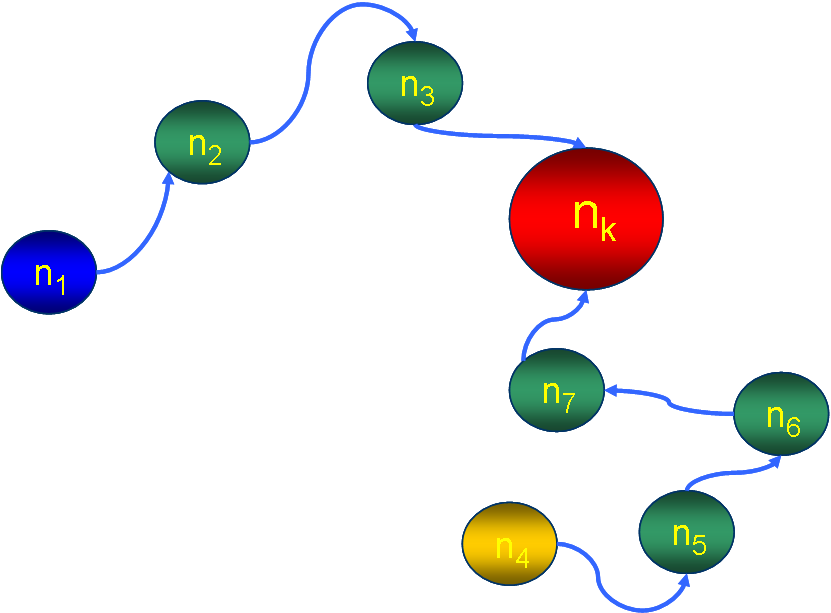
\includegraphics[width=8cm]{images/prize-sa}
    \caption{Premiando caminos \textit{Spreading Activation}}
 \label{fig:prize-sa}
\end{figure}
  
  
  

\medskip
\begin{definition}
Sea $p_i$ el número de caminos que comienzan y terminan en nodos
diferentes de $\Phi$\footnote{La recompensa no se aplica a los nodos
que pertenecen a $\Phi$.} que pasan por el nodo $c_i$ y sólo
contienen nodos pertenecientes a $\mathcal{G}$. Esta mejora asigna
un nuevo valor de activación a cada nodo $c_i$ denotado por $I^*_i$
y se calcula a través de la función $g$:
\end{definition}



\begin{equation}
I^*_i = g(I_i,p_i)
\end{equation}

En nuestro caso, tras varias pruebas la definición de la función $g$
ha sido la siguiente:

\begin{equation}
g(x,y) = x (\log(y+1)+1)
\end{equation}


\subsubsection{Algoritmo}

A continuación, el \textit{pseudocódigo }de \textit{SA}:

\begin{algorithm}
\caption{\textit{Spreading Activation}}
\begin{algorithmic}
  \REQUIRE $\Phi \neq \emptyset$  
  \ENSURE $\mathcal{G} \neq \emptyset$
  \STATE $\mathcal{A} \leftarrow \Phi$
  \STATE $\mathcal{G} \leftarrow \emptyset$
  \WHILE{$\mathcal{A} \neq \emptyset$ AND $card(\mathcal{G}) < \mathcal{G}_{\min}$ AND $N_k \ge N_{\min}$}
	\STATE $n_k \leftarrow  extraer(\mathcal{A})$
	\STATE $\mathcal{G} \leftarrow \{n_k\} \cup \mathcal{G}$	  	
	  \FORALL{$n_i / w_{ki} > 0$}	  	
	  	\STATE $N_i \leftarrow N_i + w_{ki}N_k$	
		\STATE $\mathcal{A} \leftarrow (\{n_i\} \cup \mathcal{A}) - \mathcal{G}$		
	    \ENDFOR
  \ENDWHILE
 \RETURN $\mathcal{G}$
\end{algorithmic}
\end{algorithm}

\subsubsection{Evaluación del Algoritmo}
En todo algoritmo que se precie se debe realizar un estudio tanto de la
complejidad temporal como espacial. Las consideraciones de diseño de algoritmos
están descritas en el documento ``Diseño'', no obstante se considera este
documento más apropiado para realizar una evaluación de la complejidad temporal
y espacial del algoritmo.  Atendiendo la pseudocódigo propuesto podemos
establecer las siguientes cotas:
\begin{description}
\item[Complejidad Temporal:] la ejecución del algoritmo es iterativa y su
condición de parada depende la evaluación de las restricciones. De cualquier
forma, se puede establecer como cota superior de tiempo de ejecución
$T(n)=K*C*N$, siendo $K$ una constante escalar que indica el número de
operaciones elementales a realizar para evaluar las restricciones, $C$ una
constante escalar para indicar el número de operaciones elementales necesarias
para realizar la activación de un concepto, $N$ el número de conceptos máximo
de conceptos a propagar, que en general también será escalar y aceptando que el
tiempo de ejecución para obtener la descripción de un concepto es también lineal. 

Por tanto, podemos establecer una complejidad temporal total de $T(N)$. Esta
medida, como se puede comprobar puede variar, imaginemos que cuando
seleccionamos un concepto a propagar y para obtener su descripción ejecutamos un
proceso remoto del cual no tenemos constancia de su complejidad temporal nuestra
cota en este caso no es válida. Así que en general, realizar el análisis de
complejidad temporal utilizando la teoría clásica que supone la ejecución del
algoritmo como un proceso atómico no se adapta al estudio del algoritmo,
probablemente, la complejidad temporal se ajustará más a la definida para un
\textit{crawler}, pero tampoco representa una medida adecuada ya que en la
mayoría de los casos resulta excesiva. En conclusión, tanto en el caso mejor
como en el medio (la mayoría de los casos) la complejidad temporal será lineal y
tan sólo llegaremos a una complejidad temporal de orden exponencial en el caso
de hacer una implementación muy ambiciosa en cuanto a propagación y que requiera
procesos pesados para la obtención de descripción de los conceptos.
\item[Complejidad espacial:] el estudio del espacio utilizado por el algoritmo
es mucho más sencillo y la podemos establecer en un orden máximo (para el pseudocódigo) de
$O(2*N)$, $2$ proveniente del número de conjuntos mínimo para ejecutar el
algoritmo $\mathcal{G}$ y $\mathcal{A}$, $N$ unión del número de conceptos
iniciales,propagados y activados. Implementaciones más ricas en cuanto a la
información a almacenar de los conceptos puede convertir la complejidad espacial
en $O(K*N)$ siendo $K$ el número de listas en los que puede aparecer un concepto
(para almacenar información) $N_i$ y $N$ el valor definido anteriormente.
\end{description}

En estas condiciones de complejidad, podemos afirmar que la complejidad temporal
dependen en buena medida del tiempo de acceso a la base de conocimiento para la
descripción de conceptos ya que el proceso de activación es simpre lineal. En
cuanto a la complejidad espacial será siempre del orden $N$, anteriormente definido.

En la imagen\ref{fig:proceso-sa}, se puede ver el proceso genérico de \textit{SA}.

  \begin{figure}[h]
 \centering
 %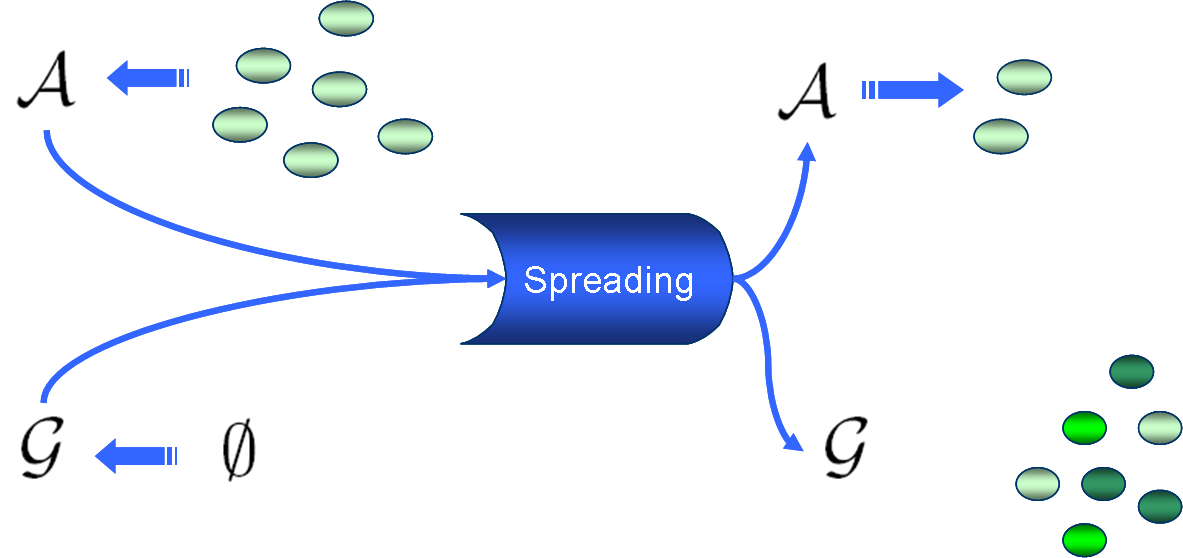
\includegraphics[width=10cm]{images/proceso-sa}
    \caption{Proceso genérico de \textit{Spreading Activation}}
 \label{fig:proceso-sa}
\end{figure}


\subsection{Casos de uso y escenarios}
La aplicación del algoritmo \textit{SA} en el ámbito de la Web Semántica puede
ser muy amplio si afrontamos su uso como un modelo para valorar el acceso a
recursos desde otro recurso determinado. Como ya hemos comentado, no se trata de
un algoritmo óptimo para la resolución de problemas, pero en cambio son buenas
técnicas para la realización de sugerencias, facilitar la realización de
ciertas tareas o comportarse como un ``ayudante'' a modo que lo haría un experto
humano. 

A continuación, comentaremos algunos escenarios en los cuales las técnicas de
\textit{SA} pueden ser aplicables.

\subsubsection{Servicios Web Semánticos}
Los SWS ampliamente comentados en la sección, se realizan
ejecutando diferentes tareas en el proceso de ejecución de global. La primera de
esas etapas es el ``descubrimiento'' o \textit{discovery}, la tarea de esta
etapa es a partir de una consulta de usuario o de un ``goal'' de ejecución
encontrar los servicios web que se adapten a las necesidades especificadas. Los
estudios sobre las técnicas de descubrimiento son amplios, ya que la
satisfacción de los objetivos del usuario empieza por tener un buen criterio
tanto en el reclutamiento de servicios web potencialmente válidos como en la
selección del servicio web a ejecutar.

Actualmente, se contemplan tres propuestas o enfoques para llevar a
cabo el descubrimiento:
\begin{description}
\item[Palabras clave:] a cada servicio web se le asocian una serie de
descriptores a través de un propiedad no funcional como \textit{subject} de
Dublin Core. Mediante un proceso de \textit{matching} entre las palabras clave
introducidas por el usuario o el ``goal'' a ejecutar se genera una lista de los
servicios web posibles. Además, si el procedimiento de reclutamiento es capaz de
valorar el servicio web de acuerdo a los descriptores de entrada y de los suyos
propios la lista puede estar ordenada por relevancia. Este método es totalmente
sintáctico (puede apoyarse en WordNet) y será tan bueno como el proceso de
valoración entre las palabras de clave de entrada y los descriptores asociados
al servicio web.
\item[Semántico \textit{lightweight} o ``simple'':] este procedimiento se basa en
utilizar
descripciones similares tanto en los objetivos como en los servicios web. El
modelado formal, usando ontologías, tanto del ``goal'' como del ``web service'' se realiza
siguiendo una metodología que genere estructuras similares para ambas entidades
(relaciones, nombres, etc.)
con el objetivo de que durante el proceso de descubrimiento se busquen estas
similaridades estructurales de forma lógica (parecido a la operación \textit{alignment} sobre
ontologías) para reclutar aquellos servicios web
 que son capaces de obtener el ``goal'' pretendido. Este procedimiento es capaz
 de clasificar los servicios en: \textit{NoMatch} (no válido), \textit{Pmatch}
 (parcialmente válido) o \textit{Match} (válido). Resumiendo, básicamente busca
 que la capacidad del servicio web coincida (explícitamente) con el objetivo
 marcado en el ``goal''.
 
 \item[Semántico \textit{heavyweight} o ``complejo'':] extiende el modelo
 anterior añadiendo nuevas relaciones a cumplir para que un servicio pueda ser
 seleccionado según un determinado ``goal''. Se basa en teoría de conjuntos y
 busca entre las posibles relaciones del servicio para determinar si de alguna
 manera puede atender a ese ``goal'' estableciendo los siguiente niveles de
 encaje: \textit{Exact-Match} o perfecto, \textit{Subsumes-Match},
 \textit{Plugin-Match} e \textit{Intersection-Match}, en estos tres últimos
 casos el problema se reduce a una serie de operaciones sobre las ontologías que
 definen al ``goal'' y al servicio web para determinar si potencialmente la
 capacidad del servicio puede conseguir el objetivo definido. Resumiendo, busca
 que la capacidad del servicio web coincida (explícita o implícitamente mediante
 relaciones con otros servicios) con el objetivo marcado en el ``goal''.
\end{description}

Podemos observar como las técnicas de encaje de servicios web de acuerdo a un
``goal'' no es una tarea sencilla, si se hace semánticamente. Por ello, creemos
que las técnicas de \textit{SA} pueden ayudar a decidir si la capacidad de un
servicio web puede atender un determinado ``goal''. Pensemos en que la entrada
del algoritmo es un conjunto de conceptos que determinan el objetivo a
conseguir. Si estos objetivos están formalizados en una ontología a través de
conceptos y relaciones, podríamos utilizar un proceso de \textit{SA},
ajustándolo correctamente, para obtener un conjunto de conceptos ponderados
generando un ``goal'' enriquecido para ser utilizado en los procedimientos
anteriormente definidos de descubrimiento semántico. De esta manera, aunque no se provee
directamente un encaje perfecto, si se provee un mecanismo para informar al
proceso de descrubrimient,o con el objetivo de mejorar la calidad de los
resultados y acotar las posibilidades de ``matching'', ya que ahora la entrada es
un conjunto de conceptos ponderados. 


\subsubsection{Clasificaciones estándar de productos}
Las clasificaciones estándar de productos representan grandes
bases
de conocimiento cuya consulta puede resultar tediosa para cualquier usuario,
incluso cuando posea una visión global de la misma. La utilización de
\textit{SKOS Core} como modelo para estas clasificaciones pueden facilitar su
consulta y explotación utilizando las técnicas de \textit{SA} de dos formas:
\begin{description}
\item[Catálogos virtuales:] en este escenario, una empresa puede tener como
vocabulario controlado para sus productos y servicios una de estas
clasificaciones para ser utilizada por distintas aplicaciones, desde la gestión
de suministros hasta aplicaciones finales de usuario. Supongamos que existe una
aplicación que permite consultar ciertos productos a partir de una consulta de
usuario, lo habitual será mostrar aquel producto o servicio que coincida
exactamente con la petición realizada pero en estas condiciones podríamos
utilizar \textit{SA}, actuando sobre la base de conocimiento, para generar una lista de
sugerencias posibles y facilitando la labor del usuario. La aplicación de esta
técnica confiere un carácter más inteligente a la aplicación ya que si la
consulta realizada no coincide exactamente con ningún producto o servicio se
generarían igualmente resultados. En caso, de que dispongamos de un conjunto de
entrada las sugerencias provistas por el algoritmo serían mucho más ajustadas,
dado un producto podríamos generar los servicios asociados con ese producto,
adelantando posiblemente la siguiente acción del usuario. 

\item[Recuperación de documentos:] una de las aplicaciones fundamentales de
estas clasificaciones es la anotación de documentos. Aunque se aplique esta
técnica, el interés de esta función recae sobre la posibilidad de recuperar los
documentos marcados con determinados términos o conceptos. Las consultas para
extraer los documentos pueden realizarse mediante un proceso automático, por
ejemplo para el reclutamiento de empresas para un contrato de licitación: una
empresa se declara como proveedora de una serie de servicios y productos, las
licitaciones están anotadas con una lista de servicios y productos. Un algoritmo
sencillo de descubrimiento sería capaz de reclutar a las empresas que son
capaces de atender a una determinada licitación agilizando el procedimiento de
concurrir al concurso. Ahora bien, si la operación a
realizar es la de consulta de documentos podemos utilizar \textit{SA} para
enriquecer y mejorar la extracción de documentos, comportándose el algoritmo
como un ayudante para buscar documentos (licitaciones). 
\end{description}

\subsubsection{Contextualización del usuario}
En este escenario, \textit{SA} puede aportar a las aplicaciones un factor humano
que mejora la experiencia de usuario. Supongamos una aplicación que utilice un
perfil de usuario en el que están definidas las preferencias del usuario de
acuerdo a la base de conocimiento, ontologías, de la aplicación. Si utilizamos esta
información del perfil como conjunto de entrada a \textit{SA} podemos mejorar la
interacción con el usuario con la aplicación apoyada en esa base de
conocimiento. Por ejemplo, en una visita virtual a un museo disponemos de una
aplicación que nos facilita información sobre los elementos disponibles en el
museo, si antes de iniciar la visita el usuario selecciona sus preferencias de
acuerdo a la información del museo la aplicación puede adaptarse al usuario y
servir sólo el contenido pretendido, pero si además utilizamos \textit{SA} para
realizar sugerencias y filtrar resultados posibles podemos generar una visita
totalmente personalizada para el usuario. Concretamente, un usuario define el
estilo ``realista'' en su perfil, las técnicas de \textit{SA} pueden usar esta
información no sólo para generar una visita conteniendo sólo los cuadros
realizados con este estilo sino también para mostrar otras obras que
pueden estar relacionadas con este estilo (según haya definido el experto
de dominio), creando una visita más completa. Afinando aún más, si la aplicación
utiliza un dispositivo georeferenciable las sugerencias pueden ser realizadas
según el transcurso del usuario dinámicamente. 


El uso de \textit{SA} nos proporciona un asesor ``humano''-virtual adecuado al
perfil de cada visitante.
Este comportamiento se puede exportar a todas aquellas aplicaciones en las que a
partir de un recurso se pueda acceder a otros y en las que dispongamos de un
perfil de usuario.


\subsubsection{Comentarios sobre la aplicación \textit{Spreading Activation}}
Todas estas propuestas de uso de las técnicas de \textit{SA} son tan sólo eso, ya
que se alejan bastante del objetivo del proyecto y del caso de uso del
Proyecto Bopa~\cite{bopaEstonia}, donde este algoritmo se ha probado como método para el enriquecimiento
de las consultas y, realmente, es una técnica perfectamente válida. 


  \begin{figure}[h]
 \centering
 %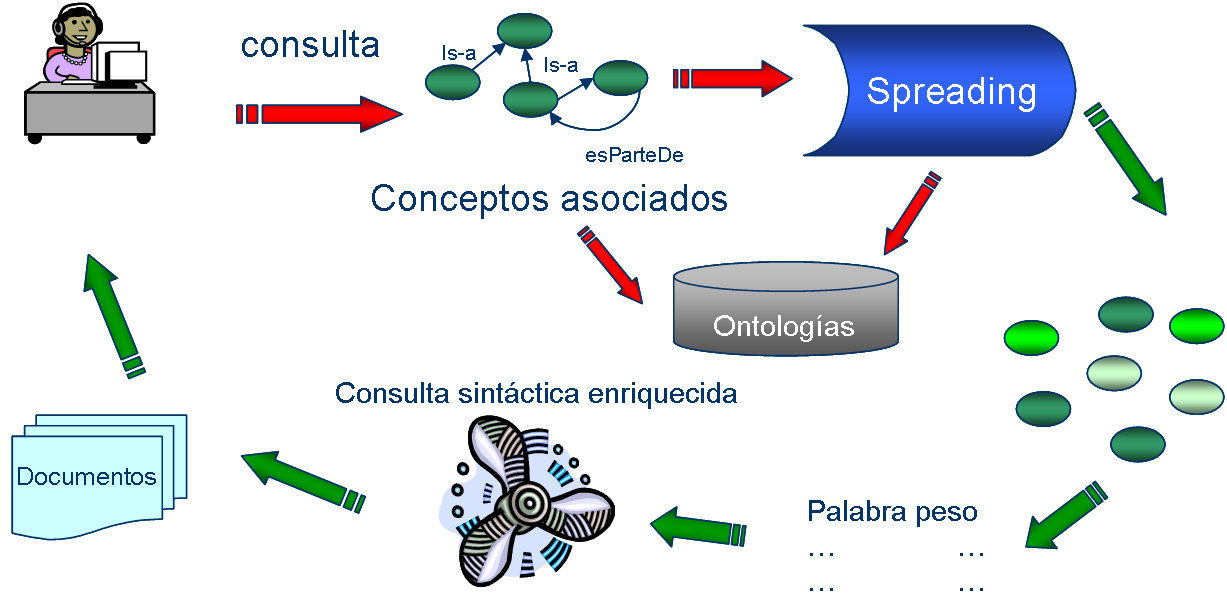
\includegraphics[width=10cm]{images/sa-search}
    \caption{Aplicando \textit{Spreading Activation} en el Proyecto Bopa}
 \label{fig:sa-search}
\end{figure}
  

No obstante, parece interesante comentar las posibilidades de aplicación a
diferentes ámbitos de la Web Semántica en los que parece hace falta ``humanizar'' la
ejecución automática.



